a%
% To start the document, use
%  \levela{...}
% For lover level, sections use
%  \levelb{...}
%  \levelc{...}
%
\levela{ARTS: concept and the programme}
 \label{sec:concept}

%
% Document history, format:
%  \starthistory
%    date1 & text .... \\
%    date2 & text .... \\
%    ....
%  \stophistory
%
\starthistory
  000616 & Created by Stefan Buehler, based on my DPG2000 poster.\\
  011121 & Practical hints added by Stefan Buehler.
\stophistory

%
% Symbol table, format:
%  \startsymbols
%    ... & \verb|...| & text ... \\
%    ... & \verb|...| & text ... \\
%    ....
%  \stopsymbols
%
%

%
% Introduction
%
This section describes the basic ideas underlying the ARTS programme.
It also introduces some terminology. You should read it if you want to
understand how the program works and how it can be used efficiently.
At the end of the chapter, there is also some practical information
about useful command line parameters and such things.



\levelb{Enter: ARTS}
%===================
\label{sec:concept:arts}

The most important notion in ARTS is the \emph{workspace}. All
physical quantities (for example absorption coefficients) are
\emph{workspace variables}. But workspace variables can also be of
a more technical nature, for example various grids. 

The program performs a calculation by executing a list of
\emph{workspace methods}, which are specified in a
controlfile. These workspace methods take workspace variables as
input, and generate workspace variables as output. Additional
input parameters can be specified as \emph{keyword parameters} in
the controlfile (Figure \ref{fig:method}).

\begin{figure}
  \begin{center}
    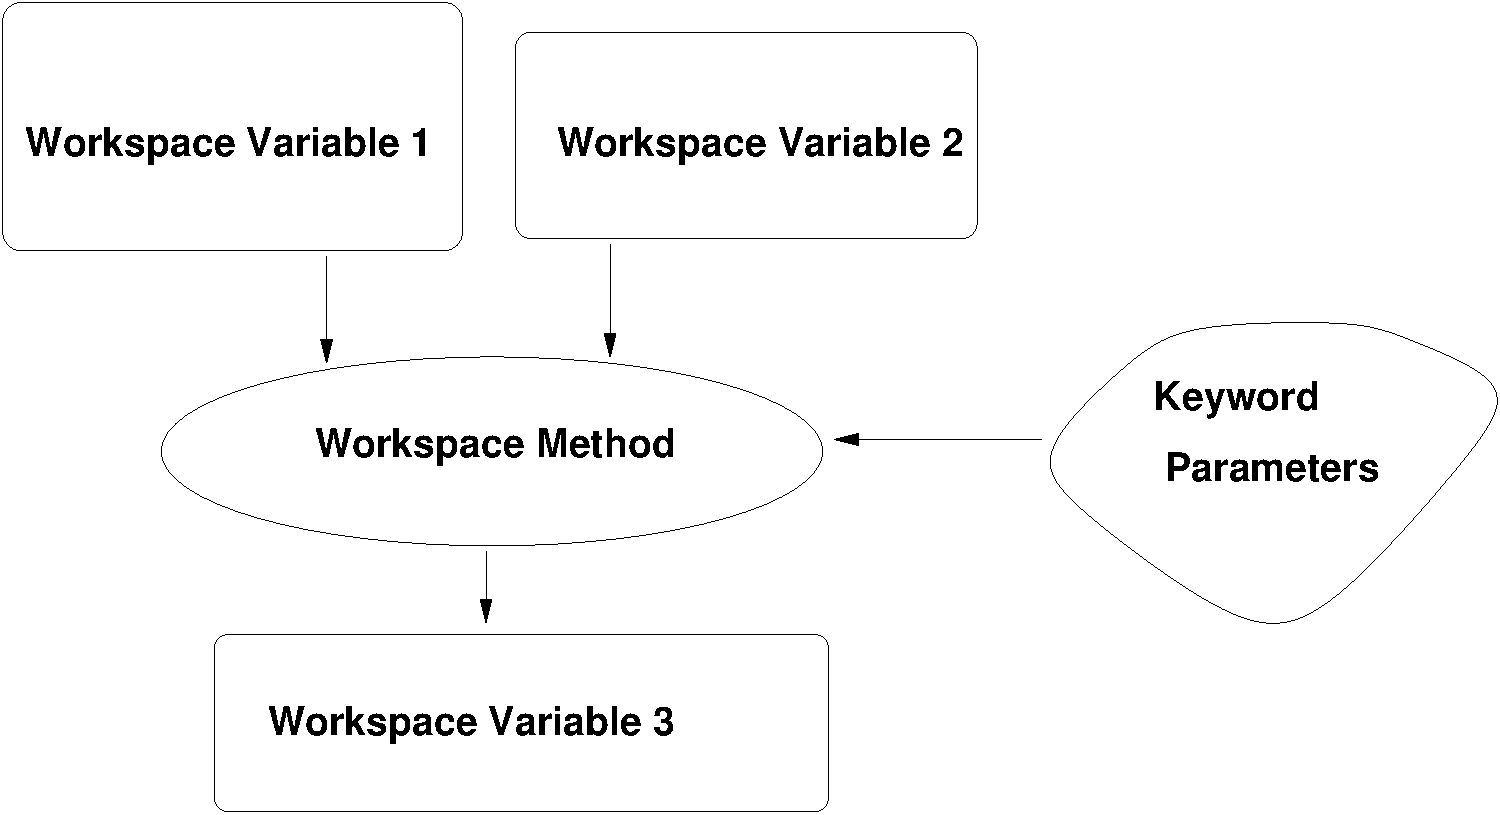
\includegraphics[width=\hsize,draft=false]{method}
    \caption{\emph{Specific}
        workspace methods act on specific workspace variables to
        generate other specific workspace variables. Additional input
        parameters can be specified as keyword parameters in the
        controlfile.}
    \label{fig:method}
  \end{center}
\end{figure}

It is important to note that the controlfile has a fixed and
well-defined syntax. This syntax is understood by the ARTS parser.
The great advantage of this concept is that it is very easy to add
new workspace variables and new workspace methods. The program has
an internal lookup table which lists all workspace methods, as well
as their input variables, output variables, and keyword
parameters. To add a new method, one just has to add an entry to
this lookup table, and write the code for the method itself. No
further changes to the program are necessary. In particular, no
changes to the program logic or to the parser. How such an extension
can be made practically is described in Section \ref{sec:development}.


\levelb{Generic Workspace Methods}
%=================================
\label{sec:concept:generic}

Generic methods (Figure \ref{fig:generic_method}) allow the user of the
program even more freedom than specific methods. A generic method is
for example \verb|VectorReadAscii|, which can be used to read any
workspace variable which is a vector from an ASCII file. For example
\begin{quote}
  \verb|VectorReadAscii(f_mono){"freqeuency_grid.aa"}|
\end{quote}
will read the specified file and generate the workspace variable
\verb|f_grid|.

\begin{figure}
  \begin{center}
    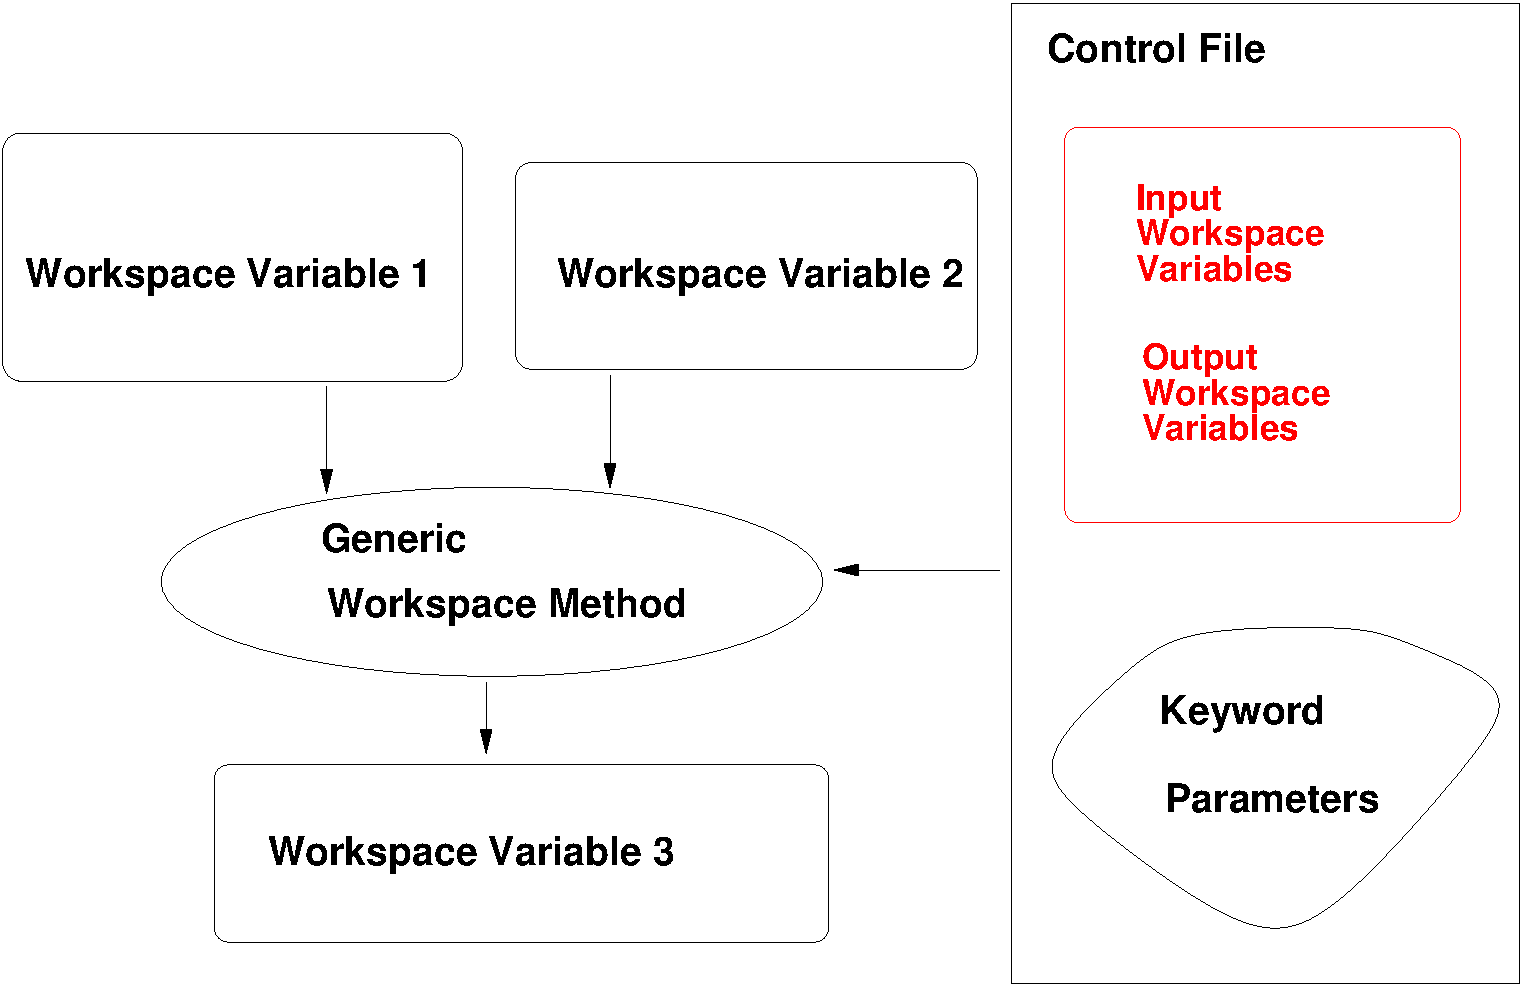
\includegraphics[width=\hsize,draft=false]{generic_method}
    \caption{For \emph{generic}
      workspace methods the workspace variables to act on are
        specified in the controlfile.}
    \label{fig:generic_method}
  \end{center}
\end{figure}

Generic methods are particularly useful for IO operations like in the
example above. No new IO functions are necessary for new workspace
variables, as long as they are of standard types already known to the
program (for example vectors or matrices). 

\levelb{Practical hints}
%=================================
\label{sec:concept:practical}

The subdirectory \verb|examples| of the \verb|doc| directory contains
some example controlfiles. You should study them to learn more about
how the program works. You can also run these controlfiles like this:
\begin{quote}
\begin{verbatim}
  arts absorption_example.arts
\end{verbatim}
\end{quote}
This assumes that you are inside the directory where the controlfiles
are, and that the \verb|arts| executable is in your path.  You can
also run all of the examples, by saying
\begin{quote}
\begin{verbatim}
  make check
\end{verbatim}
\end{quote}

ARTS offers a number of useful command line parameters. In general,
there is a short form and a long form for each parameter. The short
form consists of a minus sign and a single letter, whereas the long
form consists of two minus signs and a descriptive name. To get a full
list, type
\begin{quote}
\begin{verbatim}
  arts -h
\end{verbatim}
\end{quote}
or
\begin{quote}
\begin{verbatim}
  arts --help
\end{verbatim}
\end{quote}
Most useful at the beginning should be the \verb|-d|
(\verb|--describe|), \verb|-m| (\verb|--methods|), \verb|-w|
(\verb|--workspacevariables|), and \verb|-i| (\verb|--input|) flags.
For instance, the \verb|-d| (\verb|--describe|) flag gives you online
documentation for any workspace method or workspace variable. Usage:
\begin{quote}
\begin{verbatim}
  arts -d f_mono
\end{verbatim}
\end{quote}
will print documentation about the workspace variable \verb|f_mono|, which
happens to be the monochromatic frequency grid.

But what methods and variables are available? You can find out by
typing
\begin{quote}
\begin{verbatim}
  arts -m all
\end{verbatim}
\end{quote}
which will list all workspace methods, or by typing 
\begin{quote}
\begin{verbatim}
  arts -w all
\end{verbatim}
\end{quote}
which will list all workspace variables. As you can see, these lists
are quite long. But you can get more specific information:
\begin{quote}
\begin{verbatim}
  arts -m f_mono
\end{verbatim}
\end{quote}
will give you a list of all methods that can generate the workspace
variable \verb|f_mono|. Specific and generic methods are listed
separately. Generic methods are in this case all methods producing a
Vector, since \verb|f_mono| belongs to this group. A similar task is
performed by the \verb|-i| (\verb|--input|) flag, with the difference
that \verb|arts -i f_mono| will list those methods that require
\verb|f_mono| as \emph{input}, whereas \verb|arts -m f_mono| lists
those that produce \verb|f_mono| as output. Finally,
\begin{quote}
\begin{verbatim}
  arts -w absCalc
\end{verbatim}
\end{quote}
will give you all variables required by the method \verb|absCalc|
(the variable \verb|f_mono| happens to be one of them).

Using these command line parameters, it is easy to build up a
controlfile. The trick is, to start at the end. Say you want to
compute absorption coefficients. First of all, you have to find out
in which workspace variable these are stored. Look at the list
produced by \verb|arts -w all|. You can use \verb|arts -d| to look at
some candidates a bit more closely. This way, you will find out that
\verb|abs| is the variable you are looking for.

In the next step, you can use \verb|arts -m abs| to find all methods
that can calculate \verb|abs|. So, you will find the method
\verb|absCalc|. Now you can use \verb|arts -w absCalc| to find out the
required input variables of that method. Then you can use the
\verb|-m| flag again, to find the methods producing these variables,
and so on.

%%% Local Variables: 
%%% mode: latex
%%% TeX-master: "uguide"
%%% End: 
